\chapter{SYSTEM DESIGN}

\section{Use Case Model (Current Project)}
\begin{figure}[htbp]
    \centering
        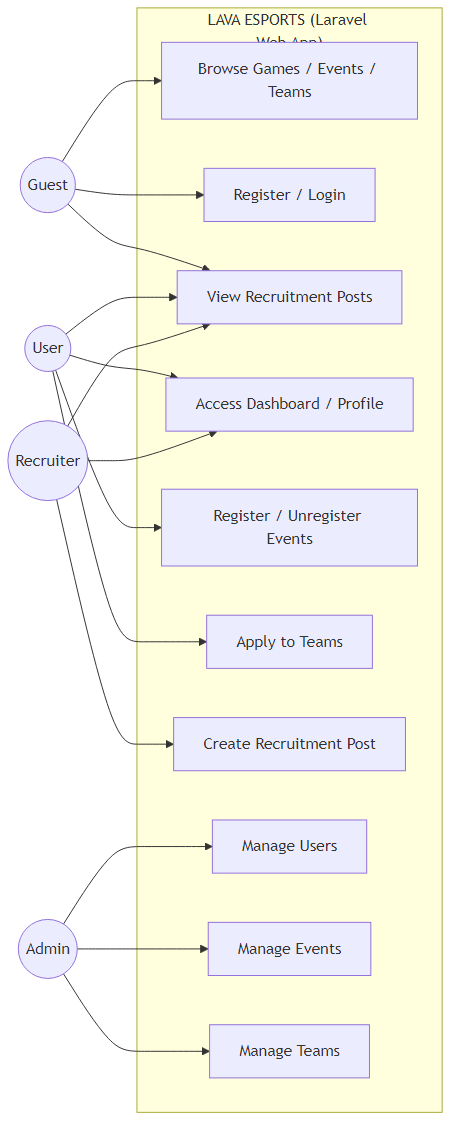
\includegraphics[width=\textwidth,height=0.85\textheight,keepaspectratio]{use_case_diagram.png}
    \caption{Current Project Use Case Diagram}
    \label{fig:use_case_current}
\end{figure}
\textbf{Diagram Explanation:} This diagram is derived from current routes and role checks. Guests can browse public content and authenticate. Authenticated users can register for events and apply to teams. Recruiters can publish recruitment posts. Admin users can manage users, events, and teams.

\section{Activity Diagram}
\subsection{Authentication and Role Routing}
\begin{figure}[htbp]
    \centering
        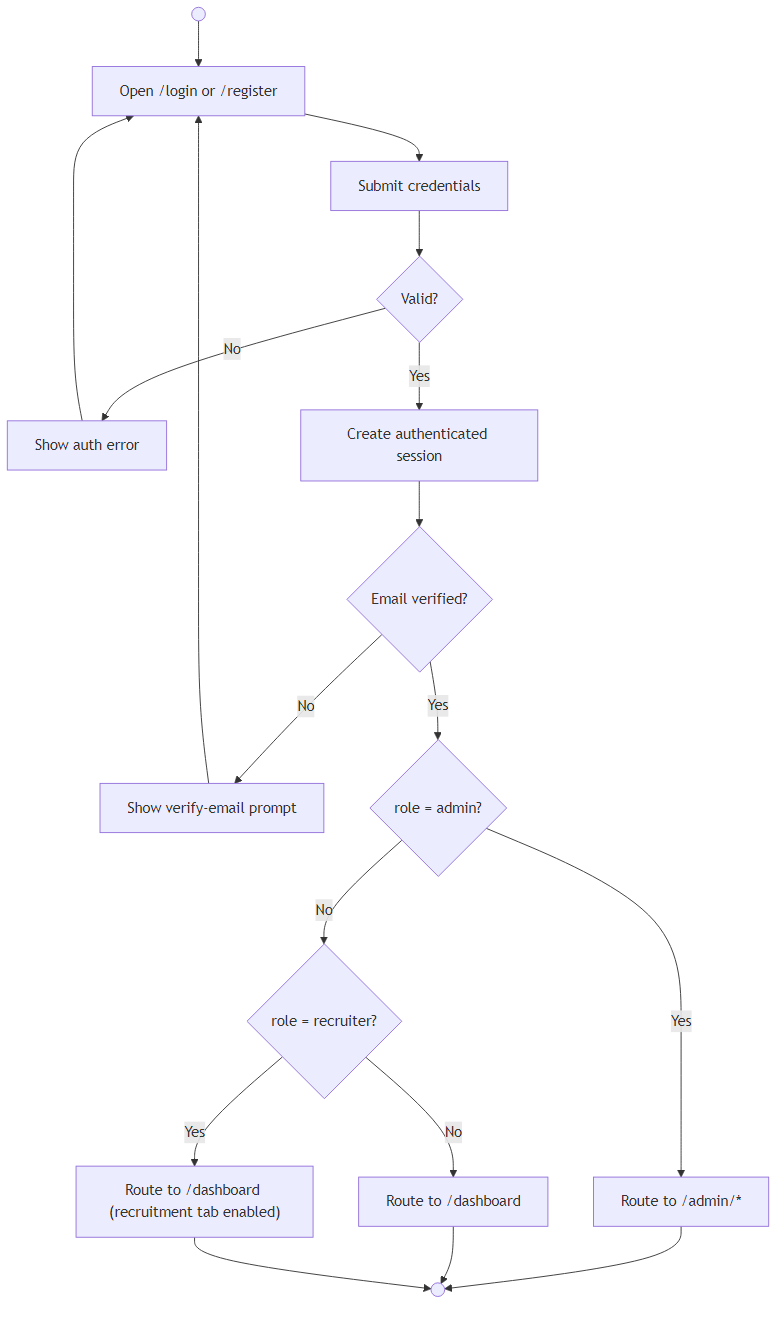
\includegraphics[width=\textwidth,height=0.4\textheight,keepaspectratio]{auth_activity_diagram.png}
    \caption{Authentication and Role-Based Routing Flow}
    \label{fig:auth_role_flow}
\end{figure}
\textbf{Diagram Explanation:} This reflects the active middleware and route structure: authenticated and verified users are routed by role, with admin-only access protected by admin middleware and recruiter capabilities gated by recruiter checks.

\section{System Architecture Diagram}
\begin{figure}[htbp]
    \centering
        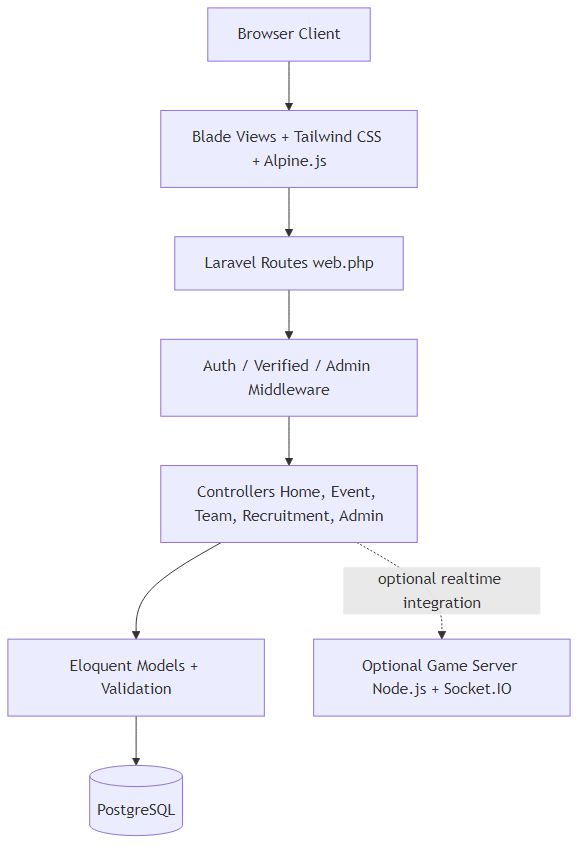
\includegraphics[width=\textwidth,height=0.85\textheight,keepaspectratio]{architecture_diagram.png}
    \caption{Current Project Architecture}
    \label{fig:architecture_current}
\end{figure}
\textbf{Diagram Explanation:} The platform is a server-rendered Laravel application where requests flow from routes through middleware and controllers to Eloquent models and PostgreSQL. An optional Node.js service can support extended real-time modules.

\section{Entity Relationship Diagram}
\begin{figure}[htbp]
    \centering
        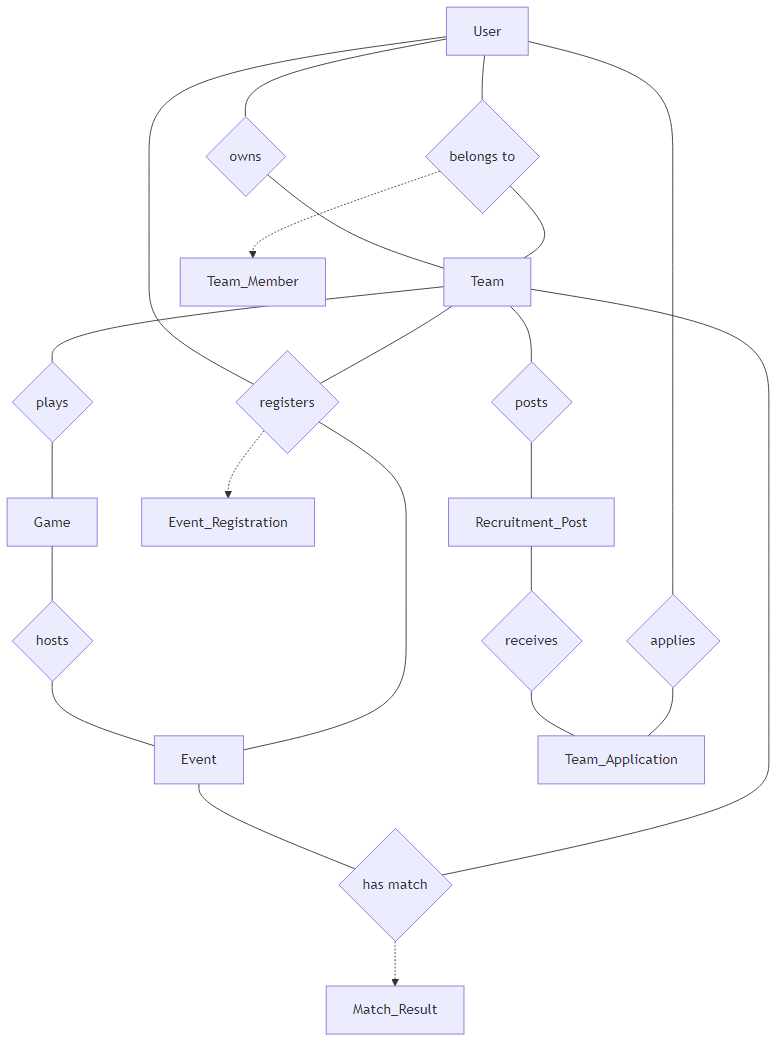
\includegraphics[width=\textwidth,height=0.85\textheight,keepaspectratio]{er_diagram.png}
    \caption{Entity Relationship Diagram}
    \label{fig:er_diagram}
\end{figure}
\textbf{Diagram Explanation:} This diagram illustrates the core entities within LAVA ESPORTS. Users can own Teams, which in turn post Recruitment listings and register for Events. Games serve as the fundamental entity linking Teams and Events.

\section{Sequence Diagram}
\subsection{Team Application Flow}
\begin{figure}[htbp]
    \centering
        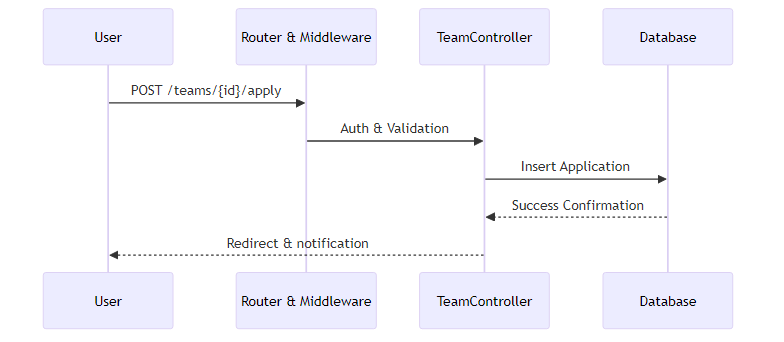
\includegraphics[width=\textwidth,height=0.85\textheight,keepaspectratio]{sequence_diagram.png}
    \caption{Sequence Diagram: Team Application Flow}
    \label{fig:sequence_diagram}
\end{figure}
\textbf{Diagram Explanation:} This sequence diagram demonstrates the interaction during a team application. A user submits a request which passes through routing and middleware for authentication. The controller processes the request and interacts with the database, returning a success response back to the user.

\section{Class Diagram}
\begin{figure}[htbp]
    \centering
        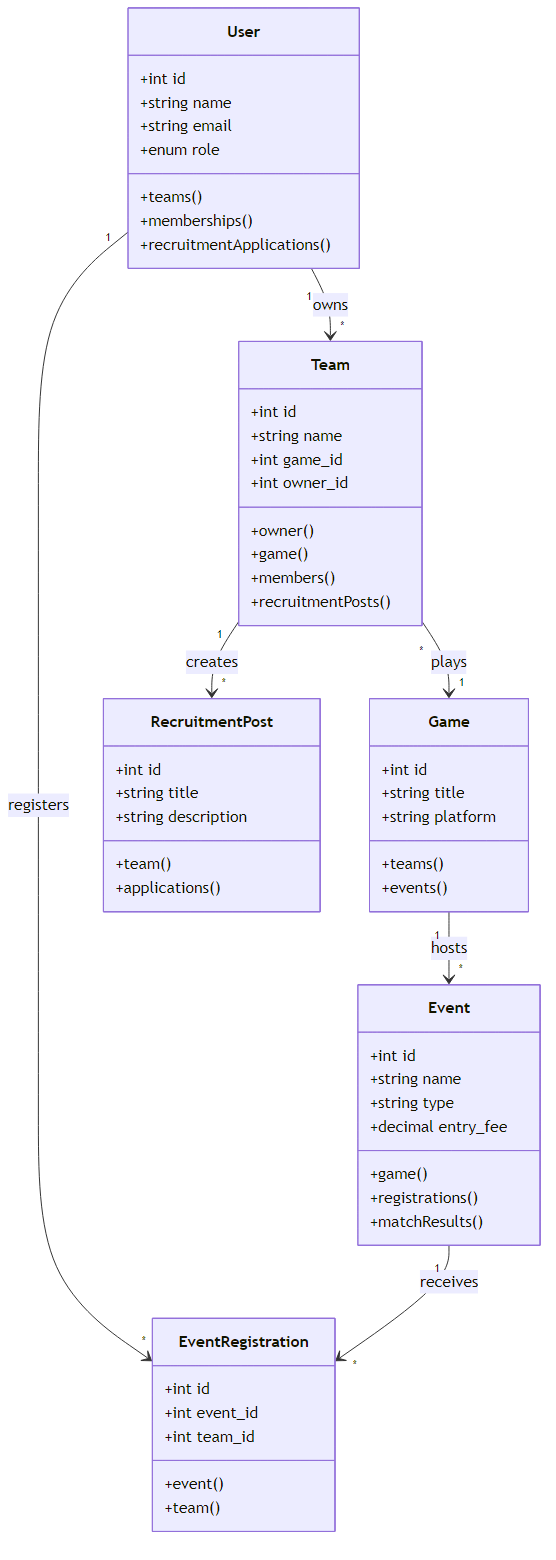
\includegraphics[width=\textwidth,height=0.85\textheight,keepaspectratio]{class_diagram.png}
    \caption{Class Diagram representing core Models}
    \label{fig:class_diagram}
\end{figure}
\textbf{Diagram Explanation:} This class diagram outlines the static structure of the core Eloquent models. It shows attributes like names and ID, and methods representing relationships such as a User belonging to a Team or an Event.

\section{Project Design Notes}
The current implementation prioritizes modularity through MVC separation and role-gated route groups. Public pages (\texttt{/games}, \texttt{/events}, \texttt{/teams}, \texttt{/recruitment}) are separated from authenticated dashboards and admin-prefixed management endpoints.

\subsection{Security Design}
Security controls in the current codebase include CSRF protection, hashed passwords, auth middleware, email verification checks on dashboard routes, and explicit admin authorization middleware for privileged actions.
